\documentclass[conference]{IEEEtran}
\usepackage{cite}
\usepackage{amsmath}
\usepackage{algorithmic}
\usepackage{url}
\usepackage{graphicx}
\usepackage{listings}
\graphicspath{ {./img/} }
% need about 4 pages full to get 4K words
\hyphenation{op-tical net-works semi-conduc-tor}
\begin{document}
\title{A Study of Identity Based Encryption Systems}

\author{\IEEEauthorblockN{Samuel Petit}
\IEEEauthorblockA{3rd Year Integrated Computer Science student at
Trinity College Dublin, the University of Dublin \\
Email: petits@tcd.ie}
}

\maketitle
\begin{abstract}
The abstract goes here.
\end{abstract}

\section{Introduction}
We will be studying the concept of Identity Based Encryption (IBE),
a type of asymmetric (or public key) encryption system which has the 
particularity of using two encryption keys, typically a public and a private key.
IBE is characterised with the fact that one of its keys identifies the recipient
(for example an email address). We will explain how such a system is possible
and compare it to a more widely known encryption scheme: RSA. Perhaps, we will
then be able to understand why IBE is not as widely used as RSA is today. 

\subsection{Introduction to Public Key Cryptography}
Public Key Cryptography, also called Asymmetric Cryptography is an 
encryption scheme. In other words, it is a method for encrypting messages.
Unlike symmetric cryptography which uses the same key for both encrypting and decrypting
messages, asymmetric cryptography uses two different keys such that one 
is used for encrypting and the other for decrypting information.
In this context, a key is a string of characters that is used in some mathematical
formula to transform information (a message for example) such that it is impossible to understand in its encrypted form. 
Similarly, we would then also use a key to map the encrypted information back to its original, usable form.
In asymmetric encryption, we typically call the encryption key
the Public Key, and the decryption key the Private Key.
The first asymmetric key cryptosystem was published in 1976 by Whitfield Diffie and Martin Hellman.
Previously, all useful modern encryption systems used symmetric key encryption systems. 
While both systems are now widely used, asymmetric key encryption systems 
have proven their potential and are now used on a daily basis throughout the world. It is implemented 
in systems such as both HTTP over TLS and HTTP over SSL protocols, digitally signed files, bitcoin,
encrypted messaging services and many others. 

\subsubsection{How it works}
Put simply, let's say we had a public key $K_{public}$ and $K_{private}$.
We would then obtain a ciphertext $cipher$ with the following formula: 
\begin{equation*}
    cipher = K_{public}(message)
\end{equation*}
Similarly, we obtain the original message from the ciphertext with the following formula:
\begin{equation*}
    message = K_{private}(cipher)
\end{equation*}


\subsubsection{Requirements for public key algorithms}
In order for a Public key encryption scheme to be safe, we have a few requirements.
The first one being ease of setup: it should be computationally easy to generate
a pair of Public and Private keys.

Encrypting a message should also be computationally easy, this means that a 
sender X, with a message to send M and knowing the recipient's public key 
should be able to compute the ciphertext fairly easily.

Similarly, decrypting a message should be computationally easy, thus meaning that
a receiver Y, with a ciphertext that was encrypted using his own public key 
should be able to obtain the original message using an easy computation.

In terms of keys, it should be impossible to obtain the private key from a 
public key, since these are, as its name suggests, public this would be a 
massive security issue.

Finally, it should also be impossible to find a message from the encrypted text and 
the public key used to obtain the ciphertext.


\subsubsection{Different implementations of Asymmetric Encryption}
Many popular protocols and systems can be used as examples of working 
asymmetric encryption. To start with, Identity Based Encryption (IBE)
uses a set of asymmetric keys. Other popular protocols or systems include
the Diffie-Hellman key exchange protocol which is used to exchange cryptographic 
keys over a non secure channel. RSA is a very popular cryptosystem which includes
algorithms and functions to compute a set of keys as well as handling encryption and decryption.
There are also multiple mathematical methods that are used by different encryption schemes,
these include  elliptic curves[1], Bilinear maps[1] or Weil and Tate Pairings[1] to name
some of the most commonly used ones.



\subsection{Introduction to Identity Based Encryption}
Identity based encryption (IBE), is a type of public key encryption 
where the public key is an arbitrary string which represents information
about a user's identity, for example, an email address. 
\subsubsection{Brief history}
The concept of using meaningful public keys dates back to 1984 where Adi Shamir
introduced the concept, it was quite a radical idea due to the fact that 
public keys are typically mathematically related to the private key. The main 
motivation for this effort was to remove the need of a public key distribution
infrastructure that is required by public key encryption schemes.
He was able to find a system for identity based signatures but was not able to 
find a working scheme for IBE itself and left it as an open question. 
It is only later in 2001 that three schemes for IBE 
were found, the two most common ones being 
found by Boneh and Franklin who's method relies on elliptic curves, and 
Clifford Cocks who's scheme relies on the RSA setting.

\subsubsection{An IBE Scheme using Elliptic Curves}
As stated previously, in a Identity Based Encryption system, 
the public key can be any arbitrary string, this fundamentally changes
from other implementations where public keys can be meaningful instead of 
a very large mathematical number. However this raises many questions such as: 
if my public key is a very simple string, how do I find the corresponding private
key to decrypt messages? and what is stopping anyone else from finding that same 
private key and decrypting my messages? Let's have a look at how IBE schemes work.


The idea involves a Private Key Generator (PKG), the PKG would be responsible 
of generating private keys for the users. It would first generate a pair of 
master keys (public key and private key). 
The master public key is used for message encryption and the master
private key is used to obtain all users' private keys.


The master public key, after its generation, would be published to all the users of the system, for a user 
to encrypt a message, he would use both the master public key and the ID of the recipient
(for example it could be an email address) to obtain the ciphertext.


Then decryption would work by using the private key associated with the ID. These are all 
computed by the PKG so the user would then have to contact the PKG and retrieve his private key,
only then is he able to decrypt the ciphertext. In order to obtain a private key from the PKG, a user 
would have to prove to the PKG that he is the owner of the key he is requesting, then the key would be sent 
through a secure channel.


Signing a message would be very similar, a user would obtain his private key from the PKG
and encrypt the message using the key and send the signature along with the ciphertext.
The recipient can then verify the signature by decrypting it using both the sender's ID and the 
master public key.


\subsubsection{Actions required by the system}
There are 4 algorithms involved in this system, these are
the \textbf{setup} algorithm which generates the pair of master public and private
keys. The \textbf{extract} action generates a private key for a public key string (for example,
generate the public key for bob's email address bob@bob.com).
Then, \textbf{encryption} is the action of obtaining the ciphertext from a message, it uses both the 
recipient ID and the master public key. Finally, \textbf{decryption} happens by decrypting the ciphertext 
using the private key generated in the extract action and the ciphertext to obtain the original message.


\subsubsection{Mathematical theory}
As mentioned previously, there are different schemes using different mathematical concepts,
let's focus here on Elliptic curve based IBE schemes. This topic involves complicated maths so 
I will try to focus on the high level mathematics theory here without 
going into too much detail.


An elliptic curve is defined by an equation of the form 
\begin{equation*}
    y^2 = x^3 + ax + b
\end{equation*}
A property of elliptic curves is that they are symmetrical about the x-axis. Here is 
a graph of a typical elliptic curve:
\begin{center}
    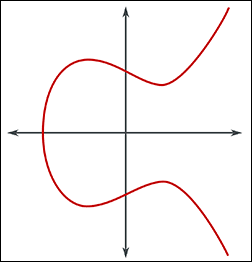
\includegraphics[scale=0.5]{ecurve}
\end{center}

The reason these
curves can be used for cryptographic purposes is thanks to the fact that, computing 
$x\*P$, where $x$ is an integer and $P$ is a point on an elliptic curve. 
We would then obtain the point Q on the curve, this is done by finding the intersection to a 
line starting from P (rember that there are an infinite number of lines that can go through a single point)
and obtaining it's symmetric point on the other side of the x axis, essentially adding P to itself, we would then do this 
operation x times in order to obtain Q.
Assuming I know the original point P, the parameters of the used curve, and the result point X, it is impossible
to obtain x (the amount of times P was added to itself).
Thus giving us a variant to the Diffie Hellman problem, which states that certain computations with 
certain groups of numbers are very easy to do one way, but very hard the other way.


Finally, it is worth noting that we can have a IBE system which uses an Bilinear map 
$e: G_{1}\times G_{1} \rightarrow G_{2}$ so long as the Computational Diffie-Hellman problem 
in $G_{1}$ is hard, meaning we can't map back to the group $G_{1}$ from $G_{2}$ then we can have a 
safe encryption system. 
One way to do so in the current elliptic curve system we are considering is to use 
the Weil pairing[2] on an elliptic curve. Ideally the bilinear map should be efficiently computable.


Let's take a look at the high level maths behind the 4 algorithms which enable 
encryption and decryption of messages using these concepts.

The setup would then pick an elliptic curve 
(in other words, a set of parameters for the elliptic curve equation), 
a secret $s$ and a point on the 
elliptic curve $P$. The system then publishes $P$ and $P\*s$ as the master public key.


Encryption would then happen by hashing the ID attribute (for example bob's email address)
to a point on the elliptic curve (let our hash function be $h = g^x$ from some x). Thus
hashing bob's ID would set $ x = ID_{bob}$. We obtain a point of the curve by doing so since $g$
is the generator for our group. Let our group be $Z_{q}^*$, of prime order q, then $g$
would be the generator for $Z_{q}^*$, this would mean that for any integer value $k$,
$g^k \in Z_{q}^*$.

Once we have hashed bob's ID, we pick a random integer $r$, an compute 
$k = e(r*h, s*P)$

We can then encrypt our message $E_{k}[M]$ using the key $k$ and send $r$ as well as the ciphertext
to the recipient.

In order to obtain the private key for a specific ID (for example, $ID_{bob}$ being bob's email address),
we need to ask the PKG for it. The PKG will
compute $s*ID$ and return the result, once again, we once again map ID to a point on the elliptic curve
using our previously mentioned hash function.
Knowing the private key for our ID, we can then decrypt 
the message by finding k first: $k = e(s*ID, r*P)$ Which will enable us to decrypt the 
ciphertext.
Note that this is possible thanks to the property for the elliptic curve that 
$e(aX, bY) = e(bX, aY)$.


It is worth noting that Cock's scheme was based on the RSA setting, we will brefly
go over RSA encryption systems in order to understand better how his scheme works.


\subsubsection{Reasons for IBE}
Now that we know more about how an IBE scheme works, let's take a look at why it exists and
what such a system enables. The first notable information is that such a system
does not need a public key distribution system, the master public key is known to all
users and thus sending an encrypted message to Bob's email address is as simple
as using the exact same email address along with the master public key for encryption. 
Meaning there is no need to manage large numbers of public keys that a typical
public key infrastructure would require.

Secondly, the central system can decrypt messages locally and because of that,
it can enable for systems with minimal setup for its users, requiring no installation 
and instead they would simply ask for the message to the central system. Note that this 
is not necessarily the best solution however it is a possibility with IBE.


Certain encrypted system require a key escrow for multiple reasons, one might be 
due to government regulations, in an IBE system, the master private key can 
generate all keys thus enabling a key escrow.

IBE also enables delegation of keys where, for example, a company employee can decrypt certain 
emails, perhaps another employee requires to read those exact same emails, the same 
private key can be used by both employees.

\subsubsection{Security of IBE}
This specific IBE scheme relies on elliptic curves with the use of 
bilinear maps thus making it follow some variant of the Diffie-Hellman problem.
That is, as of today, it is easy to compute values from operands to obtain a result,
but it is impossible to obtain the operands from the result.
For example, the use of pairings such as Weil and Tate Pairings[1] in order 
to obtain bilinear maps make it so that computing $aX$ is easy but finding $a$ 
given $X$ and $Xa$ is computationally not feasible.


Secondly, the default IBE scheme does not account for expiration of revocation of keys,
meaning that theoretically, someone obtaining a private key for a specific ID will enable 
that person to decrypt all past and future messages sent to that specific recipient.
This is very dangerous and can be avoided quite easily, one way to do so is by appending an 
expiration date to the public key, that is our ID (for example Bob's email address) and a date:
\textit{bob@bob.com \|\| <expiration date}. Bob will then be able to use that private key until 
it expires and then will have to request a new one to the PKG. The time each key is valid can 
vary based on how one decides to implement the system, theoretically a key could 
be valid for years or minutes depending on the systems capacity and its security requirements.

\subsubsection{IBE: Pushing Research Forward}
Even though identity based encryption has its flaws, it did however 
push further research in this area. From IBE was derived what is called
attribute based encryption (or ABE), a public key encryption system where the secret key is dependent 
on a users attribute (such as biometric information, country of birth...).

Both IBE and ABE were the basis for the creation of functional encryption, 
which is a generalisation of both encryption methods.


\subsection{An Overview of RSA}
Let's now see how a very popular system such as the RSA encryption scheme works, 
this will be an opportunity to understand how Clifford Cocks's RSA based scheme works.
We will then be able to compare both systems and try to understand why 
IBE is not currently commonly used.
The RSA encryption system is also a public key encryption method 
which only have 3 actions supporting it: setup, encrypt and decrypt.

\subsubsection{Key generation}
The following algorithm enables key generation:
\begin{algorithmic}
\STATE $p \leftarrow prime()$
\COMMENT{prime() returns a prime number}
\STATE $q \leftarrow prime()$
\STATE $n \leftarrow p \* q$
\STATE $\phi (n) \leftarrow (p - 1) \* (q - 1)$
\STATE $e \leftarrow coprime(\phi (n))$
\COMMENT{coprime returns a value coprime to $\phi$ where $1 < e < \phi $}
\STATE $d \equiv e^{-1} mod \phi(n)$
\end{algorithmic}
To explain a bit more about this algorithm, we start by generating randomly two prime numbers
$p$ and $q$. We obtain $n$ from their product, $n$ is used as part of the encryption and decryption function
as we will see soon. Then we use Euler's totient function such as to count the positive integers
up to $(p - 1) \* (q - 1)$ that are relatively prime to its input, we could alternatively use Carmichael's totient function here 
with a slight change in algorithm, the same keys would be generated regardless. We then pick a value $e$
such that it is positive, smaller than the value obtained from Euler's totient $\phi(n) $ function and coprime to it.
We have then obtained the public key $\{e,n\}$. To compute our private key with simply find 
the modular multiplicative inverse of e modulo $\phi(n)$ ($d \equiv e^{-1} mod(\phi(n))$) to obtain
our private key: $\{d,n\}$.

\subsubsection{Encryption}
Given a public key $\{e,n\}$, we can then very simply encrypt a message $M$.
This is done simply by computing:
\begin{equation*}
    C = M^{e}\mod n
\end{equation*}
Note that we must have $M \lt n$.
This part is fairly simple as it only contains a single operation, though keep in mind that
In practice $e$ could be a very large number so computing $M^{e}$ could be demanding on the device.

\subsubsection{Decryption}
Finally, given that we have a private key $\{d,n\}$, and a ciphertext $C$
which was encrypted using the private key's corresponding public key, we can obtain the original
message M using a formula very similar to that of the encryption:
\begin{equation*}
    M = C^{d}\mod n
\end{equation*}


\subsubsection{Security}
RSA's security relies on the fact that factoring numbers is complicated and expensive.
For instance, let's assume that we have a public key $\{e,n\}$, we could in theory find
the values for $p$ and $q$ from the key generation algorithm by factoring $n$ (recall that $n = p\*q$). Then all we would have to do is 
use Euler's theorem to obtain $\phi(n)$ and from there we could find $e$ and finally 
obtain the private key $d$ by solving the equation $e\*d = 1\mod \phi(n)$.

In practise though, we pick very large prime values for p and n, factoring very large prime
numbers is very hard and trying to obtain $p$ and $q$ using a brute force method
would be very expensive.


\subsubsection{Mathematical Theorems enabling RSA}
There are many mathematical theorems and optimisation
used in the implementation of RSA as well as RSA based encryption schemes such as 
Cock's scheme for IBE, let's now introduce some
the most common ones here.


\subsubsection*{Discrete logarithms}
The difficulty of breaking an RSA-based encryption system is based on the 
Discrete Logarithm problem (DLP). 
Given a multiplicative group $G_{n}^{*}$ of order $n$,
Let's then define the element $\alpha$ such that it is a subgroup of $G_{n}^{*}$ 
(i.e. $\alpha \subseteq G_{n}^{*}$). We then have $\alpha$, a subgroup of $G_{n}^{*}$,
note that $\alpha$ is also cyclic of order $n$ (same as $G_{n}^{*}$).


The Discrete Logarithm Problem is then defined as, given $\beta \in \alpha$,
find $x$ such that $0 \leq x \leq n - 1$.
\begin{equation}
    \alpha^{x} \equiv B\mod p
\end{equation}

It is important to note that not the discrete logarithm problem
is not always hard to solve. In the context of encryption we choose a group
$Z_{p}^*$ with $p$ a prime number which makes this problem very hard and 
expensive to solve.
It is also worth noting that not all primes are safe to use and some primes
make this problem much easier to solve, using methods such as the 
Pohlig–Hellman algorithm. In order to be safe, one can follow the rule
that a prime must be of the form $2p + 1$, where $p$ is a large prime number. 

\subsubsection*{Prime numbers}
As we have started to introduce prime numbers earlier, we can't help 
but notice that prime numbers are at the core of many concepts being
used in the types of  asymmetric encryptions we are covering here. 
There is a reason for that, it is the fact that primes are very easy to 
multiply together, however factorising a number into two prime numbers is 
extremely computer intensive. Much more so than it would be if the numbers 
weren't primes. 

So then, how do we check that a number is prime ? Do we try all possible factors
until we know we have a prime number? This approach would work, however, it 
would be terribly expensive when we are generating very large primes.
Thankfully, there are mathematical theorems we can use to make this check easier.

Two famous mathematical methods to check if a number is prime 
are Miller–Rabin and Fermat's primality test. 
Fermat's little theorem is the basis for Fermat's primality test. It states that
given, $a$, an integer and $p$ a prime number where $a$ is not divisible by $p$, we have:
\begin{equation*}
    a^{p} \equiv a (\mod p)
\end{equation*}

Thanks to this equation, we can use it to find Fermat's Primality test: 
\begin{equation*}
    a^{p - 1} \equiv 1 (\mod p)
\end{equation*}
We use it by picking two integers $a$ and $p$ such that $a$ is not divisible by $p$.
If the equality holds, then $p$ is a prime number.

The way we generate large prime numbers is by generating integers and testing if the generated integer is
prime. We can compute the probability of picking a prime number given a size. For instance if we wanted to 
find a prime number $a$ with a bit size of $2^{1024}$. We would then have a probability of picking a prime
number of \\
\begin{center}
    P(a is prime) $= \frac{2}{\ln(2^{1024})} = \frac{2}{1024\ln(2)} = 0.00281776375$
\end{center}
This probability is based on the more general Prime number theorem which statistically describes the distribution of prime numbers.
Its distribution is described as such:
\begin{equation*}
    \pi(N) \sim \frac{1}{log(N)}
\end{equation*}
Where $\pi(N)$ is the prime counting function: it computes the amount of primes
that are less than or equal to $N$.

\subsubsection*{Square and multiply}
Something you may have noticed is that some of these operations require 
computing many exponents, given the fact that we generally pick very large 
numbers for encryptions, finding a way to compute massive exponents 
in a way that is more manageable for computers would help efficient computations 
quite drastically. This is exactly what the square and multiply algorithm
enables, it is essentially an algorithm for computing exponents iteratively.
This algorithm relies on the fact that exponent value can be broken down into
the multiplication of multiple terms:
\begin{equation*}
    x^{n} =    
    \begin{Bmatrix} 
        x\*(x^{2})^{\frac{n - 1}{2}} \textrm{, if n is odd} \\
        x\*(x^{2})^{\frac{n}{2}} \textrm{, if n is even} \\  
        1 \textrm{, if n = 0} \\  

     \end{Bmatrix}
\end{equation*}


This algorithm can be implemented such that is it based on 
binary values, by using the bit values to determine which 
powers are computed.
Here is a quick example using $x^5$. $5$ in binary is $101$.
Iterating bit by bit: \\
Initialisation: result $= 1$ \\
Step 1: $\textrm{result}=\textrm{result}^2$; $(= x^0)$; bit 1 is 1; $\textrm{result} = \textrm{result}\*x$; ($= x^1$) \\
Step 2: $\textrm{result}=\textrm{result}^2$; ($= x^2$); bit 2 is 0, so there is no computation this step. \\
Step 3: $\textrm{result}=\textrm{result}^2$; ($= x^4$); bit 3 is 1, $\textrm{result} = \textrm{result}\*x$; ($= x^5$) \\

The pattern from this example is fairly straightforward, for every bit iteration, 
square our current result, then multiply by $x$ if the bit at the current position is $1$.


Note that side attacks are possible on this particular algorithm, due to 
the fact that based on the iteration being a $0$ or a $1$ a single or two
operations are executed. For instance if a hacker could access the power drawn
by the device overtime then we could notice that more power would be drawn to
compute an iteration of this algorithm with a bit value of $1$ in comparison to 
a $0$. In some cases we can monitor these from the frequencies emitted by a devie
and thus we may be able to obtain a private key using such methods.

There are ways to counter this, known as padding (explained later and add a bit here).

\subsubsection*{Chinese remainder theorem}
The chinese remainder theorem plays a big role in optimising 
the amount of work required for decrypting a message as well as 
signature verification.


Remember from the RSA setup stage that we compute 
$n = p\*q$, where n is part of the public key.
Also remember that decryption requires a ciphertext $C$ and
a private key $\{d,n\}$ to obtain the plain message $M$.
$M = C^{d}\mod n$.

We can use the Chinese remainder theorem to split the computation of
modular exponentiation, in the case of decryption using $p$ and $q$.
\begin{equation*}
    M_{P} = M\mod P
\end{equation*}
\begin{equation*}
    M_{Q} = M\mod Q
\end{equation*}
We can even push the optimisation furter:
\begin{equation*}
    M_{P} = M\mod P = (C^{d}\mod n)\mod p
\end{equation*}
\begin{equation*}
    = C^{d}\mod p\\ = C^{D\mod(P-1)}\mod p
\end{equation*}
We can do these simplifications thanks to the fact that $n = pq$ thus 
\begin{equation*}
    (C^{d}\mod n)\mod p = C^{d}\mod p
\end{equation*}
And thanks to Fermat's little theorem giving us the final optimisation.
Note that $D\mod(p - 1)$ can be computed on setup instead of during decryption
thus making this approach much faster for message decryption.

Once we have computed both $M_{q}$ and $M_{p}$, we then need to find such 
that M satisfies both:
\begin{equation*}
    M \equiv (C^{d}\mod n)\mod q
\end{equation*}
\begin{equation*}
    M \equiv (C^{d}\mod n)\mod q
\end{equation*}
Using the fact that p and q are relatively prime and because of the 
chinese remainder theorem, we can directly assume that:
\begin{equation*}
    M \equiv (C^{d}\mod n)\mod pq = M \equiv C^{d}\mod pq
\end{equation*}
Thus obtaining the decrypted message M which is what we were looking for.


\subsection{Comparisons between IBE and RSA}
Let's now go through the many pros and cons of the IBE schemes we 
have covered here and, where appropriate, compare to the functioning of the 
RSA encryption scheme.


\subsubsection{Advantages of IBE}
The first obvious advantage to IBE is the fact that we use 
meaningful public keys. This removes the need for public key distribution system
that is typically in place in most public key encryption systems. For example,
RSA typically distributes public keys using Certificate Authorities (CA), these authorities
essentially sign public keys using their own private key and return the signature. A user
can the use that signature to verify a public key is in fact the one we think it is 
and not some attackers public key for example. Put simply, 
they essentially verify the owner of the certificate, 
ensure they are who they say they are and that the provided information is valid, this
means the users put a trust in these CAs to provide accurate public keys.
In short: a key distribution infrastructure is complex, expensive and being able to 
using a public key that the user knows without looking it up is a great advantage.


Users can send messages to a recipient who has not contacted the PKG yet, meaning that 
we can encrypt messages for users who yet do not exist. This is not the case in RSA
as messages are encrypted using the recipient's public key, in order for a user to have a 
public key, that user would have to generate (so go through the setup algorithm) and 
that key would have to be inserted inside CAs databases of public keys.

If an IBE scheme accounts for private key revocation, then it is possible to enable for 
sending messages that are only decryptable at some time in the future, this is also not the 
case with RSA as keys are not generated by a central system.


We've also mentioned that message decryption can happen server-side, meaning 
this could enable applications with minimal setup for users.
 

\subsubsection{Drawbacks of IBE}
The first notable drawback is that, by definition of the 
IBE scheme we've considered, there exists a set of master
public and private keys. This means that the PKG is in a position
of generating all private keys and decrypting all messages that go through 
the system. This is known as a key escrow, it can, in some cases
be advantageous as a law may require for such a system or in an 
in an enterprise environment a key escrow may be desirable. Another
way this could be seen as an advantage is in some cases this can allow 
for recovering encrypted data in the event of the loss of a private key by a user. 
Finally, another way this is an advantage is for delegation of keys, where in some 
cases multiple persons may require to read the same messages.


However, for a public application, this requires great trust in the system 
and thus by definition is not widely adopted in systems such as 
private channels or encrypted messaging systems. The much more 
widely used RSA is much preferred in such applications, even though it requires
a key distribution system.
It is also a concern as, theoretically, if the master private key was stolen,
then an attacker would be in a position of decrypting all messages, this 
would remove all security that was previously in the system. This problem
can be solved by adding key revocation, however it is worth noting that the 
scheme we have studied here does not enable for key revocation or expiration. 
In RSA, none of this is an issue since there exists no master key that enables 
somehow the decryption of all messages, in fact, in RSA if a single key is cracked,
then only a single user will be impacted. This is also the case for IBE however,
cracking the main private key would mean the decryption of all users' messages becomes possible.
In short, IBE, by definition requires a lot of trust in the system while it is not 
the case for RSA.


Another drawback is that, in an IBE scheme, users need to be given their private key.
This can be solved by using secure communication channels, or even giving a physical copy of the 
private key on a usb key for example, however it is a drawback nonetheless since 
a private key is very sensible information (more so than a single message) and systems 
like RSA do not require to do so, a private key is generated on the device it is used.


\subsection{Attacking a Public Key Encryption system}
Many possible attacks are possible on the encryption schemes we've covered.
For example RSA, being deterministic is not very safe until we introduce concepts such as 
padding data. 

Implementations on devices of encryption or decryption methods 
can lead to security issues, for example the square and multiply algorithm,
when not randomised is prone to side attacks due to the fact that a bit value of 1 or 0 
will change drastically the time and electricity power required.

Given that such issues are dealt with, other possible attacks on the systems we've seen here include: 
Brute force, that is, trying out all the combinations in order to find the private key.

Theoretically, it could be possible to derive the private key from the public key, it just 
hasn't been proven mathematically that it is or it is not possible to do so.
We've mentioned that our schemes use the Diffie–Hellman assumption (or some variant of that assumption)
meaning that they will be safe as long as the assumption stands.

Another attack worth noting is the probable message attack, given that the public keys are known 
to attackers, one could try to encrypt all messages until there is a match.


\section{Conclusion}
We have seen that an Identity Encryption system 
introduces new concepts to the world of cryptography.
It also pushed research further by inspiring researchers
to discover what is possible from such a system where the public key is 
meaningful. One of the reasons that public key encryption systems 
were originally not widely used is due to the requirement of a public key 
distribution system, IBE solves that problem however that solution comes with 
its drawbacks. Mainly the fact that a key escrow exists by definition in the system 
without having the choice is the main drawback for IBE, it requires too much 
trust in the system for public applications. On the other hand, some argue that 
IBE is a better compromise between security and complexity for users, the main 
question being whether users see it that way or not.
Perhaps, for the moment, IBE's advantages are more suited for specific 
environments such as use within an enterprise for example.  
A lot of research is currently being done on this topic, so perhaps one day a variant 
of such an IBE scheme could become the industry standard for encryption.

\appendix
\section{Pairing Based cryptosystems}
[1]Ben Lynn June "On The Implementation of Pairing-Based cryptosystems", 
page 1 to 45.

\section{IBE Elliptic curve scheme}
[2] Dan Boneh, Matthew Franklin "Identity-Based Encryption from the Weil Pairing"

\section{RSA BASED IBE scheme}
[3] Clifford Cocks, "An Identity Based Encryption Scheme based on Quadratic Residues"

\section{Implementation}
[4] Stanford IBE Secure Email Implementation \url{https://crypto.stanford.edu/ibe/download.html}

\section{Revocable IBE}
[5] Donghoon Chang, Amit Kumar Chauhan, Sandeep Kumar, Somitra Kumar Sanadhya "Revocable Identity-based Encryption from Codes with Rank Metric"

\section{IBE without Key Escrow}
[6] Keita Emura, Shuichi Katsumata, Yohei Watanabe "Identity-Based Encryption with Security against the KGC: A Formal Model and Its Instantiations"

\section{Diffie–Hellman Assumption IBE}
[7] Nico Dottling, Sanjam Garg "Identity-Based Encryption from the Diffie-Hellman Assumption"

\end{document}


